% -*- TeX-engine: luatex -*-
\documentclass[presentation,aspectratio=43,10pt]{beamer}
\usepackage{pgfplots}
\pgfplotsset{compat=1.15}
\usepackage{template}
\renewcommand{\authorname}{Lawrence Mitchell\inst{*}}
\renewcommand{\authoremail}{\inst{*}\texttt{lawrence.mitchell@durham.ac.uk}}

\renewcommand{\sessionnumber}{8}
\renewcommand{\sessiontitle}{Roofline walkthrough + real-world code}
\usepackage{tikz}
\usetikzlibrary{matrix,fit,positioning,calc}
\usepackage{pgfplotstable}
\usepackage{booktabs}
\usetikzlibrary{pgfplots.groupplots}
\date{}

\graphicspath{{./figures/}{./figures/\jobname/}}
\begin{document}
\begin{frame}
  \maketitle
\end{frame}

\section{Generating roofline plots}

\begin{frame}
  \frametitle{Starting point}
  \begin{exampleblock}{Determine machine characteristics}
    \begin{enumerate}
    \item Measure streaming memory bandwidth using
      \texttt{likwid-bench} \texttt{triad} benchmark.
    \item[$\Rightarrow$] e.g.~for single thread \texttt{likwid-bench
        -t triad -w S0:1GB:1}
    \item Calculate peak floating point performance
      \begin{equation*}
        \text{Clock speed} \times \text{Vector width} \times
        \text{Issue width} \times \text{FMA}
      \end{equation*}
    \item On Hamilton nodes, for double precision, the vector width is
      4, it is dual issue, and does support FMA. So we have
      \begin{equation*}
        \text{Clock speed} \times 4 \times 2 \times 2 = \text{Clock
          speed} \times 16
      \end{equation*}
    \end{enumerate}
  \end{exampleblock}
\end{frame}
\begin{frame}
  \frametitle{Machine characteristics: clock speed}
  \begin{itemize}
  \item Peak clock speed is a variable, rather than fixed number
  \item For single-thread code, on Hamilton the cores can \emph{turbo
      boost} to 2.9GHz. But if they run for too long, they will be
    clocked down.
  \item[$\Rightarrow$] can put multiple lines on roofline, for base
    frequency of 2.2GHz and turbo boost of 2.9GHz
  \end{itemize}
\end{frame}

\begin{frame}[fragile]
  \frametitle{Application characteristics}
  \begin{exampleblock}{Just measure it}
    If you know the hotspot, \texttt{likwid-perfctr} can
    \emph{measure} the arithmetic intensity.

    \texttt{likwid-perfctr -g MEM\_DP ...}
\begin{minted}[fontsize=\scriptsize]{text}
...
|             DP MFLOP/s            | 1831.3403 |
|           AVX DP MFLOP/s          |         0 |
|           Packed MUOPS/s          |         0 |
|           Scalar MUOPS/s          | 1831.3403 |
...
|    Memory bandwidth [MBytes/s]    |   85.8695 |
|    Memory data volume [GBytes]    |    0.2813 |
|       Operational intensity       |   21.3270 |
\end{minted}

    Now we can plot.
  \end{exampleblock}
\end{frame}

\begin{frame}
  \frametitle{Roofline plot}
  \begin{center}
    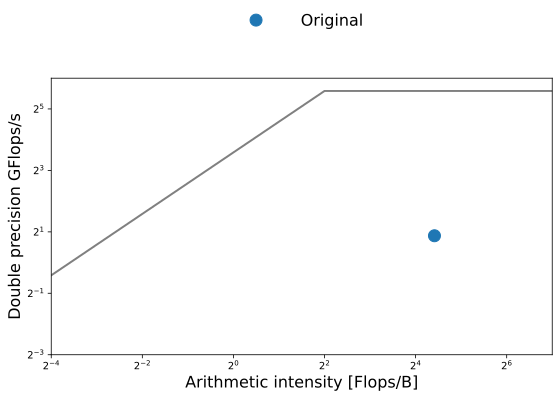
\includegraphics[height=0.9\textheight]{roofline-example-gemm}
  \end{center}
\end{frame}

\begin{frame}
  \frametitle{Application characteristics: model}
  \begin{itemize}
  \item Here it is clear that we should attempt to optimise for
    floating point throughput.
  \item We can use bounds on the data movement to bound the possible
    arithmetic intensity.
  \item Recall ``perfect cache'': each piece of data only loaded once
  \item And ``pessimal cache'': each piece of data loaded every time
  \item[$\Rightarrow$] Read code to count data access and floating
    point operations.
  \end{itemize}
\end{frame}
\begin{frame}
  \frametitle{Roofline with bounds}
  \begin{center}
    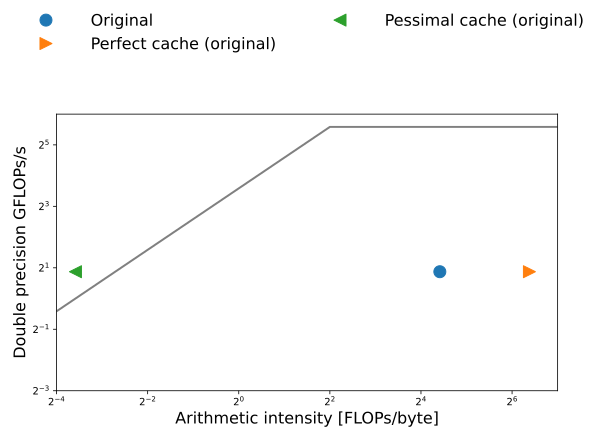
\includegraphics[height=0.9\textheight]{roofline-example-gemm-models}
  \end{center}
\end{frame}

\begin{frame}
  \frametitle{Tiling}
  \begin{center}
    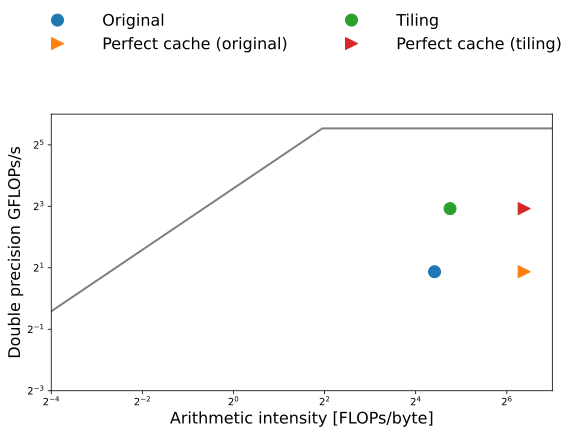
\includegraphics[height=0.9\textheight]{roofline-example-gemm-improved-tiling}
  \end{center}
\end{frame}
\begin{frame}
  \frametitle{Tiling + vectorisation}
  \begin{center}
    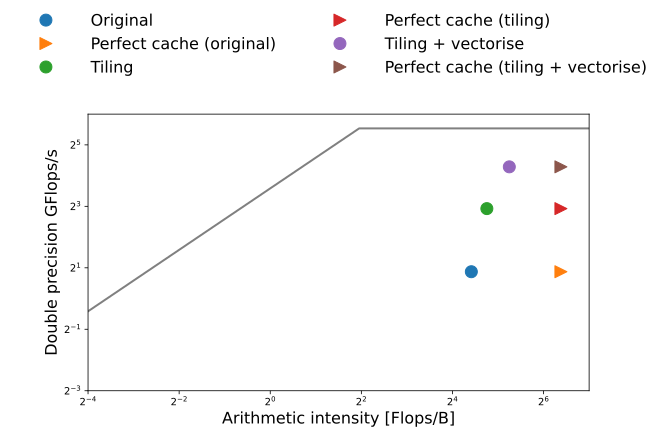
\includegraphics[height=0.9\textheight]{roofline-example-gemm-improved-tiling-vector}
  \end{center}
\end{frame}
\begin{frame}
  \frametitle{Tiling + vectorisation + compiler fiddling}
  \begin{center}
    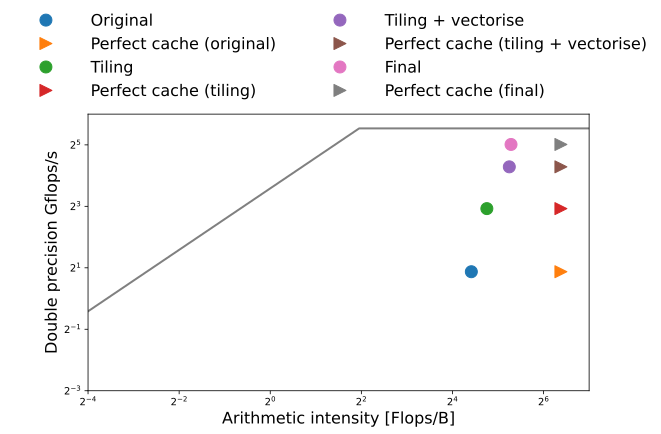
\includegraphics[height=0.9\textheight]{roofline-example-gemm-improved-all}
  \end{center}
\end{frame}


\section{Application: high performance finite elements}
\begin{frame}
  \frametitle{Application area}

  \begin{exampleblock}{Numerical solution of partial differential equations}
    Physical phenomena can be \emph{modelled} using differential
    equations.

    Example: viscous flow
    \url{https://www.youtube.com/watch?v=p08_KlTKP50}

    Modelled by Stokes' equations
    \begin{align*}
      \frac{\partial \mathbf{u}}{\partial t} -\nu \nabla^2 \mathbf{u} + \nabla p &= f\\
      \nabla \cdot \mathbf{u} &= 0
    \end{align*}

    For complicated geometries, not possible to solve with pen and
    paper $\Rightarrow$ numerical solution.
  \end{exampleblock}
\end{frame}

\begin{frame}
  \frametitle{Pictures}

  \begin{center}
    \only<1-3>{
      Freshwater mixing

      \only<1>{\includegraphics[width=\textwidth]{dome-entrainment}}
      \only<2>{\includegraphics[height=0.8\textheight]{columbia-river-unstructured}}
      \only<3>{\includegraphics[height=0.8\textheight]{thetis-snapshot}}
    }
  \only<4>{
    Chladni plates \url{https://www.youtube.com/watch?v=wvJAgrUBF4w}

    \includegraphics[width=\textwidth]{guitar-modes}
  }
  \end{center}
\end{frame}

\begin{frame}
  \frametitle{Automated finite elements}
  \begin{challenge}{Challenge}
  \begin{itemize}
  \item Simulation software needs to exploit \emph{fine-grained}
    parallelism.
  \item Most code intimately intertwines the numerical algorithm with
    its \emph{implementation}.
  \item To apply program transformations, we have to unpick,
    understand, and reimplement.
  \item \emph{Every time} the hardware changes.

  \item[$\Rightarrow$] Develop domain-specific language and
    \emph{optimising} compilers for this language.
  \end{itemize}
  \end{challenge}
\end{frame}

\begin{frame}
  \frametitle{Firedrake \url{www.firedrakeproject.org}}
  \begin{quote}
    {\normalfont [\ldots]} an automated system for the solution of
    partial differential equations using the finite element method.
  \end{quote}
  \begin{itemize}
  \item Written in Python.
  \item Finite element problems specified with embedded domain
    specific language.
  \item Domain-specific optimising compiler.
  \item Runtime compilation to low-level (C) code.
  \end{itemize}
\end{frame}
\begin{frame}
  \frametitle{Finite elements I}
  \begin{align*}
    F(u) = 0 \text{ in $\Omega$}\\
    \text{+ boundary conditions}
  \end{align*}
  Seek weak solution in some space of functions $V(\Omega)$.

  Now we need to solve the (infinite dimensional) problem, find $u\in V$ s.t.
  \begin{equation*}
    \int_\Omega \!F(u) v\, \text{d}x = 0 \quad \forall\, v \in V
  \end{equation*}
  Choose finite dimensional subspace $V_h \subset V$, find $u_h \in V_h$ s.t.
  \begin{equation*}
    \int_\Omega \!F(u_h) v_h\, \text{d}x = 0 \quad \forall\, v_h \in V_h
  \end{equation*}
\end{frame}
\begin{frame}
  \frametitle{Finite elements II}
  \begin{overlayarea}{\textwidth}{0.5\textheight}
    \only<1>{Divide domain $\Omega$\dots
    \begin{center}
      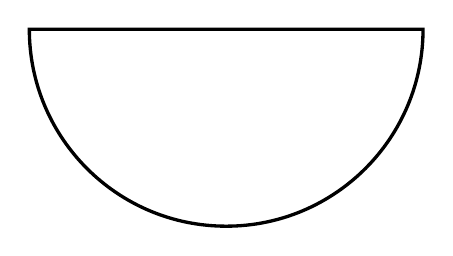
\begin{tikzpicture}
        \draw[very thick, line cap=rect] (0,0) -- (5, 0) (0, 0) arc
        (180:360:2.5);
      \end{tikzpicture}
    \end{center}}
  \only<2>{\dots{}into triangulation $\mathcal{T}$\dots
    \begin{center}
        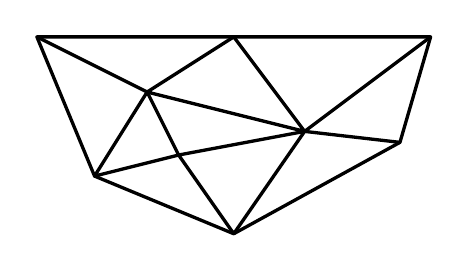
\begin{tikzpicture}
          \path (0,0) arc[radius=2.5, start angle=180, end angle=360]
          node[name=E,pos=0,swap] {} node[name=F,pos=0.25,swap] {}
          node[name=G,pos=0.5,swap] {} node[name=H,pos=0.82,swap] {}
          node[name=I,pos=1,swap] {};
          \node (A) at (2.5, 0) {};
          \node (B) at (1.4, -0.7) {};
          \node (C) at (3.4, -1.2) {};
          \node (D) at (1.8, -1.5) {};

          \draw[color=black, very thick, line cap=butt, line
          join=round] (E.center) -- (A.center) -- (I.center) --
          (H.center) -- (G.center) -- (F.center) -- (E.center) --
          cycle; \draw[color=black, very thick, line cap=butt, line
          join=round] (E.center) -- (B.center) -- (D.center) --
          (F.center) -- (B.center); \draw[color=black, very thick,
          line cap=butt, line join=round] (G.center) -- (D.center) --
          (C.center) -- (G.center); \draw[color=black, very thick,
          line cap=butt, line join=round] (B.center) -- (A.center) --
          (C.center) -- (B.center); \draw[color=black, very thick,
          line cap=butt, line join=round] (H.center) -- (C.center) --
          (I.center);
        \end{tikzpicture}
    \end{center}
  }
  \only<3>{\dots{}and choose basis with finite support.
    \begin{center}
        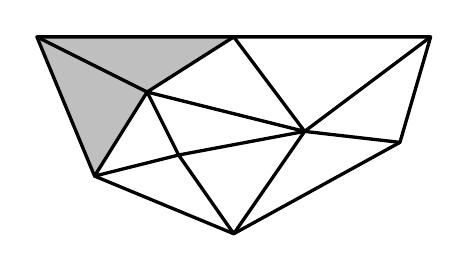
\begin{tikzpicture}
          \path (0,0) arc[radius=2.5, start angle=180, end angle=360]
          node[name=E,pos=0,swap] {} node[name=F,pos=0.25,swap] {}
          node[name=G,pos=0.5,swap] {} node[name=H,pos=0.82,swap] {}
          node[name=I,pos=1,swap] {}; \node (A) at (2.5, 0) {}; \node
          (B) at (1.4, -0.7) {}; \node (C) at (3.4, -1.2) {}; \node
          (D) at (1.8, -1.5) {};

        \path[fill=gray!50] (E.center) -- (A.center) -- (B.center) --
        (F.center) --cycle;
          \draw[color=black, very thick, line cap=butt, line
          join=round] (E.center) -- (A.center) -- (I.center) --
          (H.center) -- (G.center) -- (F.center) -- (E.center) --
          cycle; \draw[color=black, very thick, line cap=butt, line
          join=round] (E.center) -- (B.center) -- (D.center) --
          (F.center) -- (B.center); \draw[color=black, very thick,
          line cap=butt, line join=round] (G.center) -- (D.center) --
          (C.center) -- (G.center); \draw[color=black, very thick,
          line cap=butt, line join=round] (B.center) -- (A.center) --
          (C.center) -- (B.center); \draw[color=black, very thick,
          line cap=butt, line join=round] (H.center) -- (C.center) --
          (I.center);
        \end{tikzpicture}
      \end{center}
      }
  \end{overlayarea}
\end{frame}

\begin{frame}
  \frametitle{Finite elements III}
  Integrals become sum over element integrals
  \begin{equation*}
    \int_\Omega\! F(u_h) v_h \, \text{d}x =
    \sum_{e \in \mathcal{T}} \int_e\! F(u_h)v_h\, \text{d}x
  \end{equation*}

  (Usually) perform element integrals with numerical quadrature
  \begin{equation*}
    \int_e F(u_h)v_h\,\text{d}x = \sum_q w_q F(u_h(q)) v_h(q)\,\text{d}x
  \end{equation*}

  Replace $u_h(q), v_h(q)$ with expansion in finite element basis
  \begin{align*}
    u_h(q) &= \sum_i u_h^i \phi_i(q)\\
    v_h(q) &= \phi_j(q)\\
  \end{align*}
\end{frame}

\begin{frame}
  \frametitle{Challenges}
  \begin{block}{Global}
    Meshes are \emph{unstructured}, can't just use dense arrays.

    Use sparse representation, needs graph algorithms for ordering and
    partitioning of work.
  \end{block}

  \begin{block}{Local}
    Computational \emph{kernel} more complicated than simple stencil
    code.
  \end{block}
\end{frame}


\begin{frame}[fragile]
  \frametitle{A domain-specific compiler}
  \begin{columns}
    \begin{column}{0.45\textwidth}
      \begin{equation*}
        a(u, v) = \int_\Omega \nabla u \cdot \nabla v\,\text{d}x \quad \forall v \in V
      \end{equation*}
\begin{minted}[fontsize=\scriptsize]{python}
V = FiniteElement("Lagrange", triangle, 1)
u = TrialFunction(V)
v = TestFunction(V)
F = dot(grad(u), grad(v))*dx
\end{minted}
    \end{column}
    \hspace{0.05\textwidth}
    \begin{column}{0.45\textwidth}
      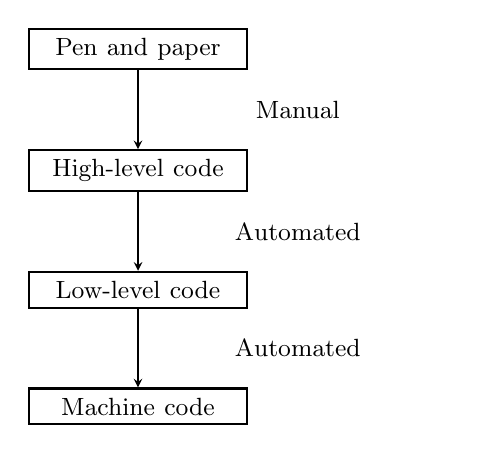
\begin{tikzpicture}
        \node[draw,rectangle, thick, text width=1in, align=center] (A)
        {\small Pen and paper};

        \node[draw, below=of A, rectangle, thick, text width=1in,
        align=center] (B) {\small High-level code};

        \node[draw, below=of B, rectangle, thick, text width=1in,
        align=center] (C) {\small Low-level code};

        \node[draw, below=of C, rectangle, thick, text width=1in,
        align=center] (D) {\small Machine code};

        \draw[-stealth] (A) -> (B) node [midway,right,text
        width=1.5in,align=center] {\small Manual};

        \draw[-stealth] (B) -> (C) node [midway, right, text
        width=1.5in, align=center]
        {\small Automated};

        \draw[-stealth] (C) -> (D) node [midway, right, text
        width=1.5in, anchor=west, align=center] {\small Automated};
      \end{tikzpicture}
    \end{column}
  \end{columns}
\end{frame}

\begin{frame}[fragile]
  \frametitle{Typical generated code}
  \begin{columns}
    \begin{column}{0.5\textwidth}
\begin{minted}[fontsize=\tiny]{c}
static inline void kernel(double A[6],
    const double *restrict coords,
    const double *restrict w_0) {
  static const double t3[12] = {...};
  static const double t4[12][6] = {...};
  double t0 = -1 * coords[0];
  double t1 = -1 * coords[1];
  double t2 =
    fabs((t0 + coords[2]) * (t1 + coords[5]) -
         (t0 + coords[4]) * (t1 + coords[3]));
  for (int ip = 0; ip < 12; ip += 1) {
    double t5 = 0.0;

    for (int i_0 = 0; i_0 < 6; i_0 += 1) {
      t5 += t4[ip][i_0] * w_0[i_0];
    }
    double t6 = t3[ip] * t2 * pow(t5, 2);

    for (int j = 0; j < 6; j += 1) {
      A[j] += t4[ip][j] * t6;
    }
  }
}
\end{minted}
    \end{column}
    \begin{column}{0.5\textwidth}
\begin{minted}[fontsize=\tiny]{c}
int execute_kernel(int start, int end,
    double *A, int32_t *Amap,
    double *coords, int32_t *coordsmap,
    double *w_0, int32_t *w_0map) {
  for (int i = start; i < end; i++) {
    double lA[6] = {0};
    double lcoords[3, 2];
    double lw_0[6];
    /* Pack into contiguous element data */
    for (int i_0 = 0; i_0 < 3; ++i_0) {
      lcoords[i_0, 0] = coords[coordsmap1[i, i_0], 0];
      lcoords[i_0, 1] = coords[coordsmap1[i, i_0], 1];
    }
    for (int i_0 = 0; i_0 < 6; ++i_0) {
      lw_0[i_0] = w_0[w_0map2[i, i_0]];
    }
    /* Execute kernel on contiguous data */
    kernel(lA, lcoords, lw_0);
    /* Scatter result */
    for (int i_0 = 0; i_0 < 6; ++i_0) {
      A[Amap[i, i_0]] += lA[i_0];
    }
  }
  return 0;
}
\end{minted}
    \end{column}
  \end{columns}
\end{frame}

\begin{frame}
  \frametitle{What does the performance look like?}
  \begin{center}
    Full node of Xeon Gold (Skylake) with AVX512 instruction set.
    \only<1>{\includegraphics[width=\textwidth]{helmholtz-roofline-before}}
    \only<2>{\includegraphics[width=\textwidth]{elasticity-roofline-before}}
    Not great.
  \end{center}
\end{frame}

\begin{frame}
  \frametitle{Cause}
  \begin{itemize}
  \item No data point gets close to roofline limits
  \item[$\Rightarrow$] Hypothesis: compilers do a bad job of
    vectorising this code.
  \item Confirmed by measuring instruction mix.
    \begin{center}
      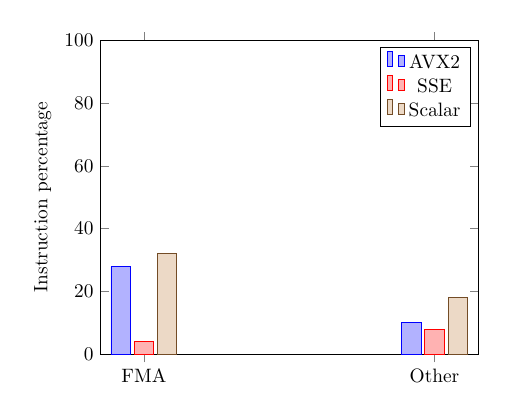
\begin{tikzpicture}[scale=0.7]
        \begin{axis}[ybar, ymin=0, ymax=100, xtick=data,
          ylabel={Instruction percentage},
          enlarge x limits=0.15,
          symbolic x coords={FMA, Other}]
          \addplot  coordinates {
            (FMA, 28)
            (Other, 10)
          };
          \addplot coordinates {
            (FMA, 4)
            (Other, 8)
          };
          \addplot coordinates {
            (FMA, 32)
            (Other, 18)};
          \legend{AVX2,SSE,Scalar}
        \end{axis}
      \end{tikzpicture}
    \end{center}
  \item[$\Rightarrow$] Need to help compiler to generate better code.
  \item Local data layout transformation.
  \end{itemize}
\end{frame}

\begin{frame}
  \frametitle{Idea}
  \begin{itemize}
  \item Enough \emph{local} work for vectorisation to be effective
  \item \dots but loop trip counts are unfriendly;
  \item \dots and loop nests are hard to analyse.
  \item To obtain nice loops, need \emph{outer loop} vectorisation and
    layout transformation
  \item[$\Rightarrow$] must do this by hand
  \item Strategy: operate on \texttt{SIMD\_WIDTH} elements at once.
  \item Dimension-lifted transposition approach, but for unstructured
    data
  \item[$\Rightarrow$] don't expect perfect speedup.
  \end{itemize}
\end{frame}

\begin{frame}
  \frametitle{Schematic: before}
  \begin{center}
    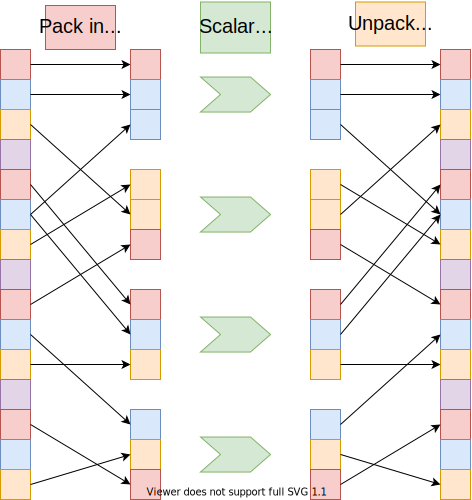
\includegraphics[height=0.8\textheight]{unstructuredtranspose}
  \end{center}
\end{frame}

\begin{frame}
  \frametitle{Schematic: after}
  \begin{center}
    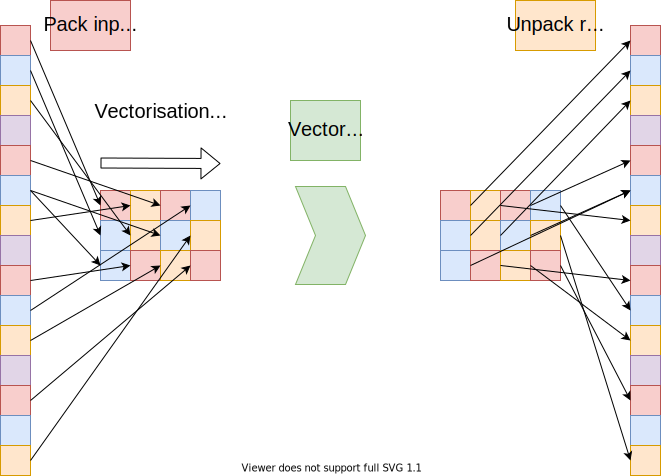
\includegraphics[height=0.8\textheight]{unstructuredtransposeafter}
  \end{center}
\end{frame}

\begin{frame}
  \frametitle{Schematic: both}
  \begin{columns}
    \begin{column}{0.45\textwidth}
      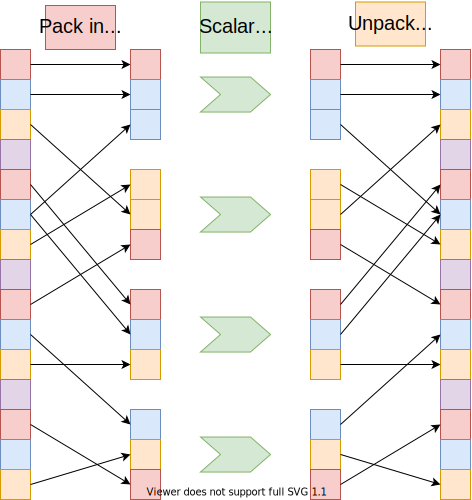
\includegraphics[width=\textwidth]{unstructuredtranspose}
    \end{column}
    \begin{column}{0.45\textwidth}
      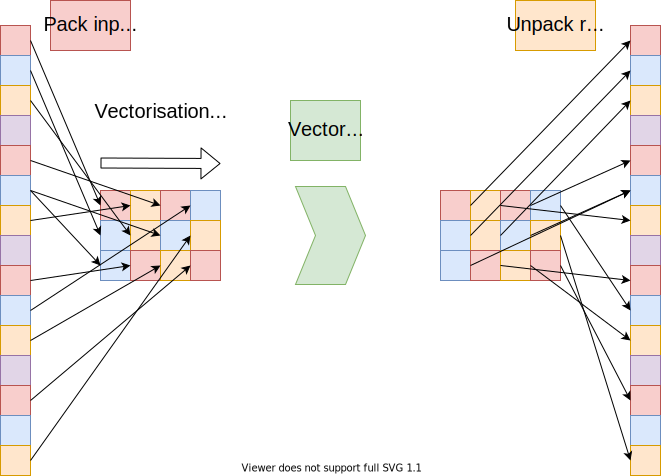
\includegraphics[width=\textwidth]{unstructuredtransposeafter}
    \end{column}
  \end{columns}
\end{frame}
\begin{frame}[fragile]
  \frametitle{Promoting vectorisation: kernel}
  \begin{columns}[t]
    \begin{column}{0.5\textwidth}
      Hard to vectorise

\begin{minted}[fontsize=\tiny, bgcolor=green!10]{c}
static inline void kernel(double A[6],
    const double *restrict coords,
    const double *restrict w_0) {
  static const double t3[12] = {...};
  static const double t4[12][6] = {...};
  double t0 = -1 * coords[0];
  double t1 = -1 * coords[1];
  double t2 =
    fabs((t0 + coords[2]) * (t1 + coords[5]) -
         (t0 + coords[4]) * (t1 + coords[3]));
  for (int ip = 0; ip < 12; ip += 1) {
    double t5 = 0.0;

    for (int i_0 = 0; i_0 < 6; i_0 += 1) {
      t5 += t4[ip][i_0] * w_0[i_0];
    }
    double t6 = t3[ip] * t2 * pow(t5, 2);

    for (int j = 0; j < 6; j += 1) {
      A[j] += t4[ip][j] * t6;
    }
  }
}
\end{minted}
    \end{column}
    \begin{column}{0.5\textwidth}
      Easy to vectorise

\begin{minted}[fontsize=\tiny,escapeinside=||, bgcolor=green!10]{c}
static inline void kernel4(double A[6, 4],
    const double *restrict coords[4],
    const double *restrict w_0[4]) {
  static const double t3[12] = {...};
  static const double t4[12][6] = {...};
  |{\setlength{\fboxsep}{1pt}\colorbox{red}{\texttt{for (int b = 0; b < 4; b++)}}}| {
    double t0 = -coords[0, |{\setlength{\fboxsep}{1pt}\colorbox{red}{\texttt{b}}}|];
    double t1 = -coords[1, |{\setlength{\fboxsep}{1pt}\colorbox{red}{\texttt{b}}}|];
    double t2 =
      fabs((t0+coords[2, |{\setlength{\fboxsep}{1pt}\colorbox{red}{\texttt{b}}}|])*(t1+coords[5, |{\setlength{\fboxsep}{1pt}\colorbox{red}{\texttt{b}}}|]) -
           (t0+coords[4, |{\setlength{\fboxsep}{1pt}\colorbox{red}{\texttt{b}}}|])*(t1+coords[3, |{\setlength{\fboxsep}{1pt}\colorbox{red}{\texttt{b}}}|]));
    for (int ip = 0; ip < 12; ip += 1) {
      double t5 = 0.0;

      for (int i_0 = 0; i_0 < 6; i_0 += 1) {
        t5 += t4[ip][i_0] * w_0[i_0, |{\setlength{\fboxsep}{1pt}\colorbox{red}{\texttt{b}}}|];
      }
      double t6 = t3[ip] * t2 * pow(t5, 2);

      for (int j = 0; j < 6; j += 1) {
        A[j, |{\setlength{\fboxsep}{1pt}\colorbox{red}{\texttt{b}}}|] += t4[ip][j] * t6;
      }
    }
  }
}
\end{minted}
    \end{column}
  \end{columns}
\end{frame}
\begin{frame}[fragile]
  \frametitle{Execution wrapper: before}
  \begin{columns}
    \begin{column}{0.5\textwidth}
\begin{minted}[fontsize=\tiny]{c}
int execute_kernel(int start, int end,
    double *arg0, int32_t *map0,
    double *arg1, int32_t *map1,
    double *arg2, int32_t *map2) {
  for (int i = start; i < end; i++) {
    double buffer0[6] = {0};
    double buffer1[3, 2];
    double buffer2[6];
\end{minted}
      \vspace{-1.2\baselineskip}
\begin{minted}[fontsize=\tiny,bgcolor=red!20]{c}
    /* Pack into contiguous element data */
    for (int i_0 = 0; i_0 < 3; ++i_0) {
      buffer1[i_0, 0] = arg1[map1[i, i_0], 0];
      buffer1[i_0, 1] = arg1[map1[i, i_0], 1];
    }
    for (int i_0 = 0; i_0 < 6; ++i_0) {
      buffer2[i_0] = arg2[map2[i, i_0]];
    }
\end{minted}
      \vspace{-2.4\baselineskip}
\begin{minted}[fontsize=\tiny,bgcolor=green!20]{c}
    /* Execute kernel on contiguous data */
    kernel(buffer0, buffer1, buffer2);
\end{minted}
      \vspace{-2.4\baselineskip}
\begin{minted}[fontsize=\tiny,bgcolor=orange!20]{c}
    /* Scatter result */
    for (int i_0 = 0; i_0 < 6; ++i_0) {
      arg0[map0[i, i_0]] += buffer0[i_0];
    }
  }
}
\end{minted}
    \end{column}
    \begin{column}{0.5\textwidth}
      \begin{center}
        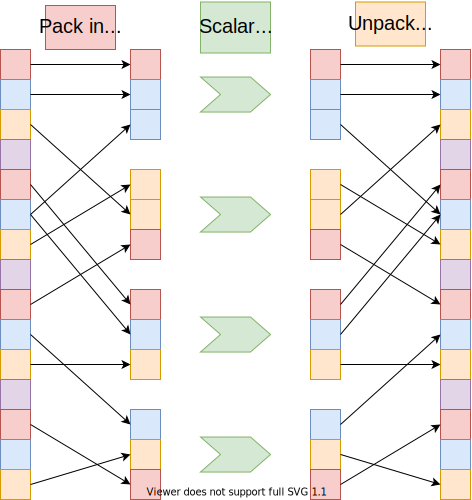
\includegraphics[width=\textwidth]{unstructuredtranspose}
      \end{center}
    \end{column}
  \end{columns}
\end{frame}
\begin{frame}[fragile]
  \frametitle{Execution wrapper: after}
  \begin{columns}
    \begin{column}{0.5\textwidth}
      \begin{center}
        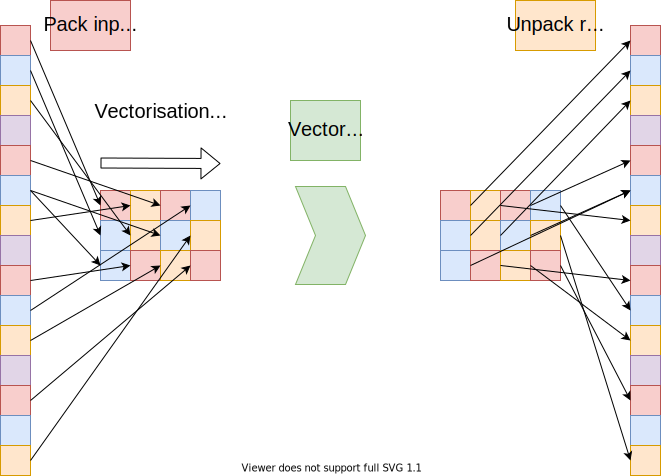
\includegraphics[width=\textwidth]{unstructuredtransposeafter}
      \end{center}
    \end{column}
    \begin{column}{0.5\textwidth}
\begin{minted}[fontsize=\tiny]{c}
int execute_kernel(int start, int end,
    double *arg0, int32_t *map0,
    double *arg1, int32_t *map1,
    double *arg2, int32_t *map2) {
  /* Stride by SIMD width */
  for (int i = start; i < end; i+=4) {
    double buffer0[6, 4] = {0.0};
    double buffer1[3, 2, 4];
    double buffer2[6, 4];
\end{minted}
      \vspace{-1.2\baselineskip}
\begin{minted}[fontsize=\tiny,bgcolor=red!20]{c}
    /* Pack four elements into contiguous data */
    for (int i_0 = 0; i_0 < 3; ++i_0) {
      for (int b = 0; b < 4; b++) {
        buffer1[i_0, 0, b] = arg1[map1[i + b, i_0], 0];
        buffer1[i_0, 1, b] = arg1[map1[i + b, i_0], 1];
      }
    }
    for (int i_0 = 0; i_0 < 6; ++i_0) {
      for (int b = 0; b < 4; b++) {
        buffer2[i_0, b] = arg2[map2[i + b, i_0]];
      }
    }
\end{minted}
      \vspace{-2.4\baselineskip}
\begin{minted}[fontsize=\tiny,bgcolor=green!20]{c}
    /* Execute kernel on contiguous data */
    kernel4(buffer0, buffer1, buffer2);
\end{minted}
      \vspace{-2.4\baselineskip}
\begin{minted}[fontsize=\tiny,bgcolor=orange!20]{c}
    /* Scatter result */
    for (int i_0 = 0; i_0 < 6; ++i_0) {
      for (int b = 0; b < 4; b++) {
        arg0[map0[i + b, i_0]] += buffer0[i_0, b];
      }
    }
  }
}
\end{minted}
    \end{column}
  \end{columns}
\end{frame}

\begin{frame}
  \frametitle{New instruction mix}
  \begin{itemize}
  \item Inner kernel annotated with \texttt{\#pragma omp simd} appropriately
  \item[$\Rightarrow$] Compilers should do a good job vectorising this
    code (stride-1 inner loop, perfect data layout)
  \item Confirmed by measuring instruction mix.
    \begin{center}
      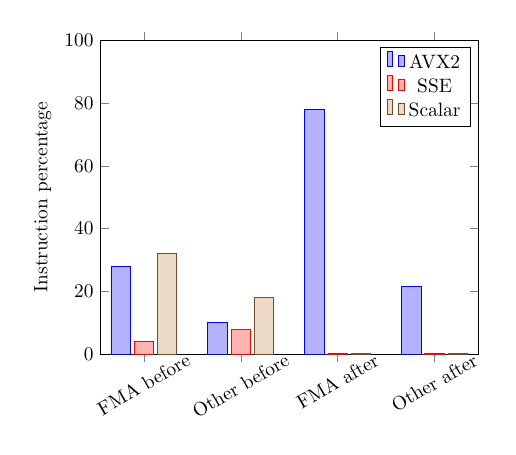
\begin{tikzpicture}[scale=0.7]
        \begin{axis}[ybar, ymin=0, ymax=100, xtick=data,
          ylabel={Instruction percentage},
          enlarge x limits=0.15,
          xticklabel style={rotate=30, yshift=0.3cm, xshift=0.17cm},
          symbolic x coords={FMA before, Other before, FMA after, Other after}]
          \addplot  coordinates {
            (FMA before, 28)
            (Other before, 10)
            (FMA after, 78)
            (Other after, 21.6)
          };
          \addplot coordinates {
            (FMA before, 4)
            (Other before, 8)
            (FMA after, 0.1)
            (Other after, 0.1)
          };
          \addplot coordinates {
            (FMA before, 32)
            (Other before, 18)
            (FMA after, 0.1)
            (Other after, 0.1)
          };
          \legend{AVX2,SSE,Scalar}
        \end{axis}
      \end{tikzpicture}
    \end{center}
  \end{itemize}
\end{frame}

\begin{frame}
  \frametitle{Performance significantly better}
  \begin{center}
    Full node of Xeon Gold (Skylake) with AVX512 instruction sets.
    \only<1>{\includegraphics[width=\textwidth]{helmholtz-roofline-after}}
    \only<2>{\includegraphics[width=\textwidth]{elasticity-roofline-after}}
    Significantly better.
  \end{center}
\end{frame}

\begin{frame}
  \frametitle{Conclusions}
  \begin{itemize}
  \item Performance now limited by combination of unstructured data
    movement and instruction throughput.
  \item[$\Rightarrow$] needs more work for further gains.
  \item More details in \arxivlink{1903.08243}{cs.MS}
  \end{itemize}

  \begin{exampleblock}{Projects using Firedrake}
    If you're interested in either numerics-based or performance-based
    projects using numerical software, come and speak to me!
  \end{exampleblock}
\end{frame}
\end{document}
